\documentclass[11pt,a4paper,pdftex]{amsart}
\usepackage[psamsfonts]{amssymb}
%\usepackage{amssymb}
\usepackage{amsmath,amsfonts,latexsym}
\usepackage{t1enc}
\usepackage[english]{babel}
\usepackage{graphicx}
\usepackage{amscd}
\usepackage{verbatim}
\usepackage{multicol}
\usepackage[utf8]{inputenc}

\newtheorem{ej}{Ejercicio}%[section] %numera os 'Ejercicios' reseteando
%en cada 'cap�tulo'.


\numberwithin{equation}{section}%numera las formulas reseteando
%cada vez que cambia de 'cap�tulo'.

\newcommand{\bej}[1]{\begin{ej}\rm{#1}}
\newcommand{\eej}{\end{ej}\vspace{-0.2cm}}
%---------------------------------------
\newcommand{\be}{\begin{enumerate}}
\newcommand{\ee}{\end{enumerate}}
\newcommand{\bit}{\begin{itemize}}
\newcommand{\eit}{\end{itemize}}
\newcommand{\bc}{\begin{center}}
\newcommand{\ec}{\end{center}}
\newcommand{\ba}{\begin{array}}
\newcommand{\ea}{\end{array}}
\newcommand{\bq}{\begin{quotation}}
\newcommand{\eq}{\end{quotation}}
\newcommand{\beq}{\begin{equation}}
\newcommand{\eeq}{\end{equation}}
\newcommand{\mc}[1]{\mathcal{#1}}
\newcommand{\mb}[1]{\;\mbox{#1}\;}
\newcommand{\su}[1]{\underline{#1}}
\newcommand{\so}[1]{\overline{#1}}
\newcommand{\ang}[1]{\widehat{#1}}
\newcommand{\arc}[1]{\wideparen{#1}}
\newcommand{\cc}{QQ\;}
\renewcommand{\bf}{\textbf}
\newcommand{\comb}[2]{\left(\!\!\!\ba{c}#1\\[1ex]#2 \ea
\!\!\!\right)}
%-----------------------------------------
%conjuntos
\newcommand{\W}{\mathbb W}
\newcommand{\K}{\mathbb K}
\newcommand{\N}{\mathbb N}
\newcommand{\C}{\mathbb C}
\newcommand{\Z}{\mathbb Z}
\newcommand{\Q}{\mathbb Q}
\newcommand{\R}{\mathbb R}
\newcommand{\F}{\mathbb F}
\newcommand{\A}{\mathbb A}
\newcommand{\V}{\mathbb V}
\newcommand{\I}{\mathbb I}
\newcommand{\0}{\mathbb O}
%------------------------------------------
%operaciones
\newcommand{\8}{\infty}
\newcommand{\ie}{\langle}
\newcommand{\de}{\rangle}
\newcommand{\pe}[2]{\ie {#1} \, ; \, {#2} \de }
\newcommand{\f}[1]{\overrightarrow{#1}}
\newcommand{\DT}[2]{\frac{d{#1}}{d{#2}}}
\newcommand{\ds}{\displaystyle}
\newcommand{\dg}{\Delta}
\newcommand{\g}{\nabla}
\newcommand{\D}{\mbox{div}}
\newcommand{\Dp}[1]{\partial_{#1}}
\newcommand{\DP}[2]{\frac{\partial{#1}}{\partial{#2}}}
\newcommand{\sen}[1]{\mbox{sen}\;{#1}}
\newcommand{\Lp}[1]{L^{#1}}
\newcommand{\To}{\longrightarrow}
%-------------------------------------
%griegos
\newcommand{\vi}{\varphi}
\newcommand{\om}{\omega}
\newcommand{\Om}{\Omega}
\newcommand{\ve}{\varepsilon}
%-------------------------
%comandos particulares
\newcommand{\id}[1]{\text{id}_{#1}}
\newcommand{\mD}{\mc{D}}
\newcommand{\mC}{\mc{S}}
\newcommand{\mS}{\mc{SS}}
\newcommand{\mH}{\mc{H}}
\newcommand{\HD}{\mc{H}_\mD}
%%%%%%%%%%%%%%%%%%%%%%%%%%%%%%%%%%%%%%%%%%%%%%%%%%%%%%%%%%%%%%%%%
%Un comando para insertar dibujos
\newcommand{\putfig}[4]{\bigskip \bigskip
             \begin{figure}[ht]
             \epsfxsize=#1cm\hfil{\epsfbox{#2}}
             \caption{#3}
         \label{#4}
             \end{figure}\bigskip}
%La sintaxis
%\putfig{ancho}{.eps}{titulo}{label}
%%%%%%%%%%%%%%%%%%%%%%%%%%%%%%%%%%%%%%%%%%%%%%%%%%%%%%%
%Un comando para insertar dos dibujos
\newcommand{\putfigg}[4]{\bigskip \bigskip
             \begin{figure}[ht]
             \epsfxsize=5cm\hfil{\epsfbox{#1}}
             \epsfxsize=5cm\hfil{\epsfbox{#2}}
             \caption{#3}
         \label{#4}
             \end{figure}\bigskip}
%La sintaxis
%\putfigg{.eps}{.eps}{titulo1}{label1}
%%%%%%%%%%%%%%%%%%%%%%%%%%%%%%
%un dibujo en jpg
\newcommand{\putjpg}[3]{\bigskip
\begin{center}
 \begin{figure}[ht]
  \hspace{5cm}\includegraphics[scale=1.7]{#1.jpg}
  \caption{#2}
  \label{#3}
  \bigskip
  \bigskip
 \end{figure}
\end{center}
}
%la sintaxis \putjpg{.jpg}{Titulo}{label}
%----------------------------------------------------
%diseñoo de la página

\vfuzz7pt % Don't report over-full v-boxes if over-edge is 7pt small
\hfuzz7pt % Don't report over-full h-boxes if over-edge is 7pt small

\pagestyle{myheadings}

\renewcommand{\labelenumi}{({\it \alph{enumi}})}
\renewcommand{\labelenumii}{\arabic{enumii})}

\flushbottom \textwidth17cm \textheight23cm \hoffset=-2cm
\voffset=-0.5cm

\begin{document}


%\markboth{}{\hfil {\sc An\'alisis II--An\'alisis matem\'atico II--Matem\'atica 3. 1er. Cuatrimestre 2008}}

\begin{center}

\bf{\Large An\'alisis II -- An\'alisis matem\'atico II -- Matem\'atica 3.} \\
\bigskip
\bf{\large Segundo Cuatrimestre de 2025}\\
\bigskip
\bf{Pr\'actica 0 - Repaso de integraci\'on y cambio de variables.}
\end{center}

\section{Principio de Cavalieri.}


\bej Considerar un cuerpo que ocupa una regi\'on $\Om$ en el espacio comprendida entre los planos $z=a$ y $z=\ell.$ Deduzca que el volumen del cuerpo se puede calcular como
$$
V = \int_a^{\ell} A(t) \, dt,
$$
donde $A(t)$ es el \'area de la secci\'on del cuerpo obtenido al intersecarlo con el plano $z=t.$
\vskip-1.7cm

\[
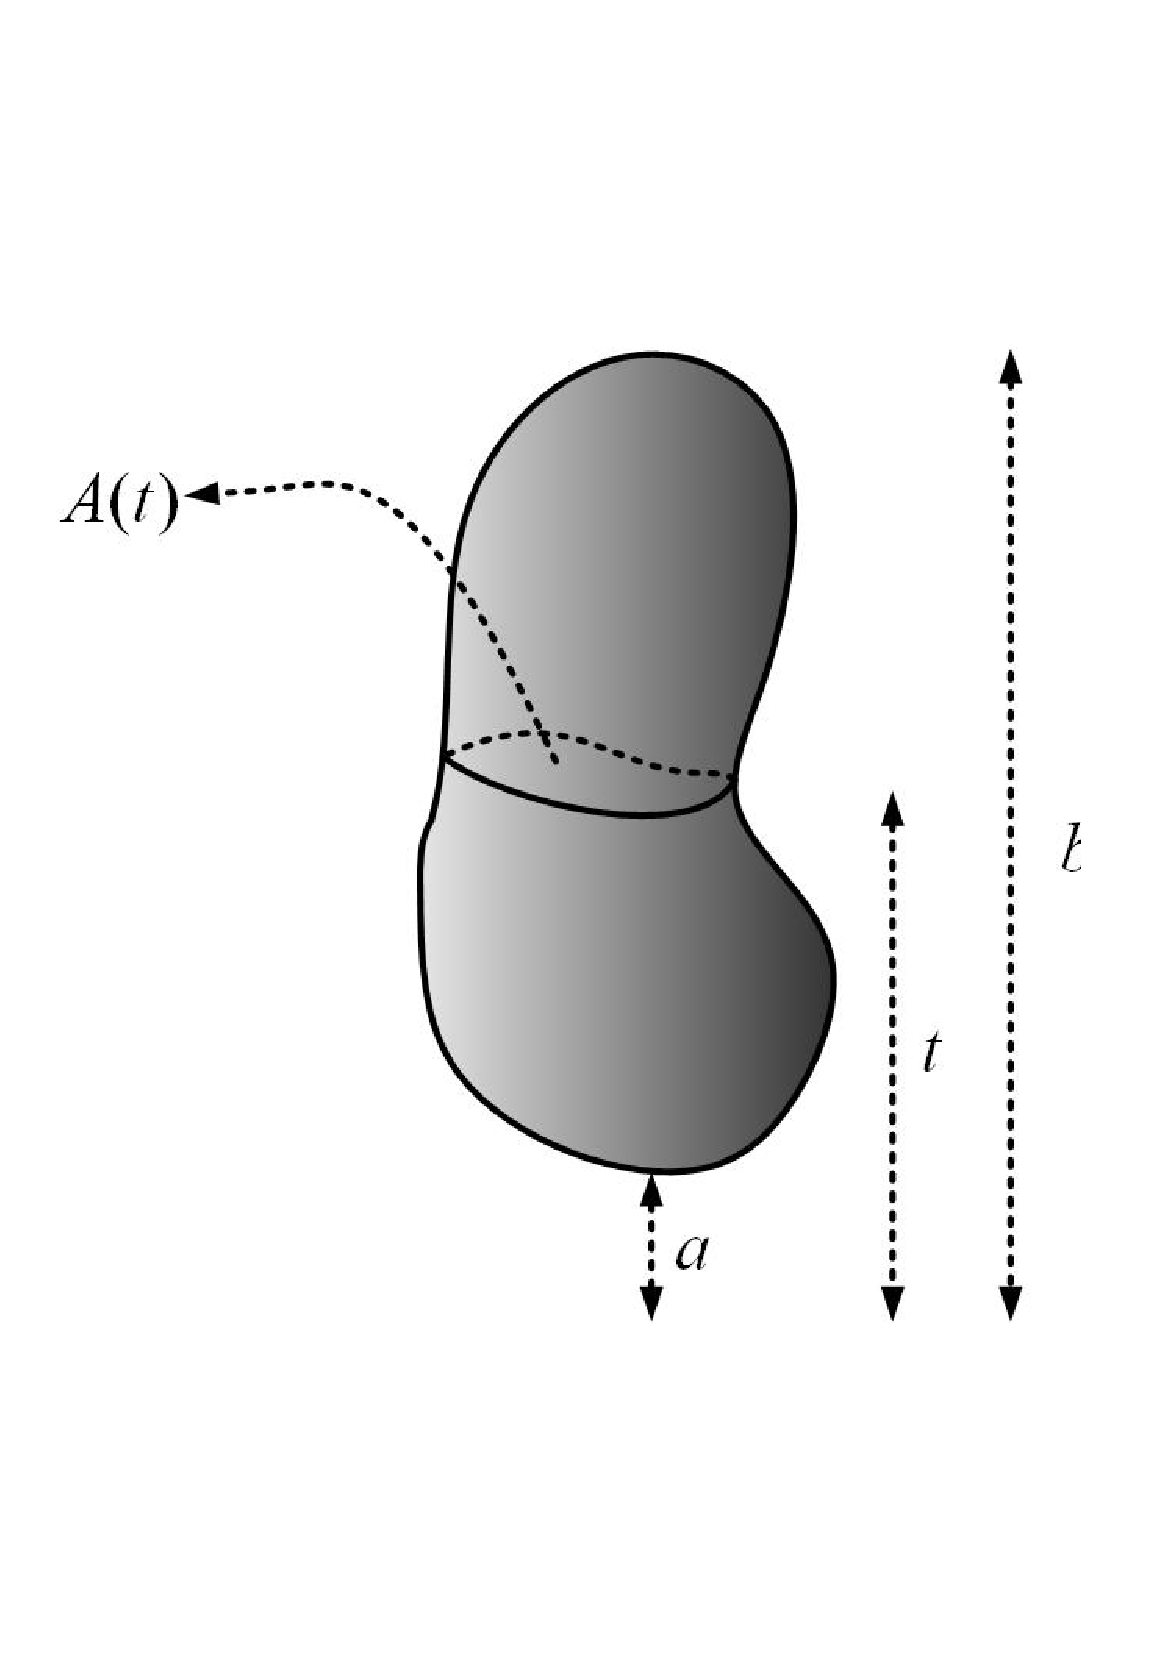
\includegraphics[width=6.5cm]{cavalieri.eps}
\]
\eej

\vskip-3cm

\bej Calcular el volumen de una regi\'on cilindr\'ica. Verificar que la f\'ormula resultante coincide con la
f\'ormula emp\'irica {\em superficie de la base por altura}.\eej



\bej Calcular el volumen de la regi\'on encerrada por el paraboloide de ecuaci\'on $z=x^2+y^2$ y el plano $z=2.$\eej



\section{Fubini.}

\bej Enunciar el Teorema de Fubini.
\eej

\bej  Sea $R$ el rect\'angulo $R=[-1; 1]\times[0;1].$ Evaluar las siguientes integrales dobles:
\begin{multicols}{2}
\begin{enumerate}
 \item $\iint_R x^2 y \,dA,$


 \item $ \iint_R x \cos(xy)\, dA,$


 \item $\iint_R \frac{xy}{1+x^2} \, dA,$



 \item $\iint_R \frac{y^n}{({1-\frac{x^2}{4})^{-\frac{1}{2}}}} \, dA.$
\end{enumerate}
\end{multicols}
\eej

\bej Sea $R$ el rect\'angulo arbitrario $[a;b]\times[c;d].$ Expresar mediante integrales simples la integral doble
$\iint_R F(x,y) \,dA$ cuando $F(x,y)$ est\'a dada por
%\begin{multicols}{2}
\begin{enumerate}
  \item $F(x,y)=f(x) g(y).$
   \item $ F(x,y)=f(x)+g(y).$
 \end{enumerate}
%\end{multicols}
\eej


\section{Descripci\'on de Regiones.}

\bej Sea $T $ el tri\'angulo de v\'ertices $(0;0),$ $(2;3)$ y $(3;5).$ Describirlo como una regi\'on de tipo 1. Describirlo como una regi\'on de tipo 2. Hallar el \'area. \eej

\bej Para cada una de las siguientes descripciones, graficar la regi\'on correspondiente y calcular el \'area respectiva.
\begin{enumerate}
\item $-1 \leq x \leq 1+y;$ \,$-1\leq y \leq 1,$
\item $0\leq y \leq \sqrt{1-x^2};$\, $0\leq x\leq 1,$

\end{enumerate}
\eej

\bej Sea $\mathcal{P}$ la pirámide cuyos vértices son $(0;0;0), (1;0;0), (0;1;0)$ y $(0;0;1)$. Describirla analíticamente. Hallar el volumen. 
\eej




\section{Aplicaciones de la integral.}
\textit{Recuerdo}: El valor medio de una función escalar $f(x)$ en una región $D \subseteq \mathbb{R}^n$ se define como:
\[
\textit{M.V} \ (f) = \frac{1}{\text{Vol}(D)} \int_D f(x) \, dx,
\]
si una región $D$ tiene una densidad $\rho(x)$ que varía en el espacio, la masa $M$ de la región se puede calcular integrando la densidad sobre $D$. Esto se expresa como:
\[
M = \int_D \rho(x) \, dx.
\]
\bej {\em Valor medio:} hallar el valor medio de la funci\'on $f(x,y)=x^2 y$ en la regi\'on triangular de v\'ertices $(1;1);$ $(2;0)$ y $(0;1).$ \eej

\bej{\label{masa}} {\em Masa:} hallar la masa de la regi\'on esf\'erica $x^2+y^2+(z-R)^2=R^2$ sabiendo que la
densidad de masa es proporcional a la componente $z,$ digamos $\varrho=\lambda z.$ \eej



\section{Cambio de Variables.}

\bej Enunciar el Teorema de Cambio de Variable. 
\eej

\bej {\label{cvl}} Sean $T(u,v)=T(x(u,v),y(u,v))=(a_{11}u+a_{12}v,a_{21}u+a_{22}v)$ con
$a_{ij}\in \R$. Sea $D^*$ el rectángulo $[0,3]\times[1,3]$.
\begin{enumerate}
\item Hallar $D=T(D^*)$. ¿Es  biyectiva $T$?  Observar que $D$ es un paralelogramo y  hallar su área.
\item Describir el área de $D$ en términos de una integral sobre $D^*$. Indicar que función hay que integrar y  que relación tiene con $T$.

\end{enumerate}
\eej

\bej Sea
 %$T(u,v)=(4u+v,2u+3v)$ y
$D$ el paralelogramo de vértices $(1,2),\,(5,3),\,(2,5),\,(6,6)$.
%$D=T(D^*)$ con $D^*=[0,1]\times[1,2].$.
Calcular
 \begin{enumerate}
  \item $\int_D xy\,dxdy$
   \item $\int_D(x-y)\,dxdy$
 \end{enumerate}

\eej


\bej
Sean $D^{*}=\{(r,\theta ):0\le r\le 1; \,\,\, 0\le \theta \le 2\pi \}$, $%
D=\{(x,y):x^2+y^2\le 1\}$ y $P$ la transformaci\'{o}n de coordenadas polares
a cartesianas, es decir, $P(r,\theta )=(x(r,\theta ),y(r,\theta ))=(r\cos
\theta ,r\sin \theta )$.
\begin{enumerate}
\item Demostrar que $P(D^{*})=D$.\thinspace \textquestiondown Es biyectiva $P$?
\item \textquestiondown En qu\'e transforma $P$ el rect\'{a}ngulo $[r,r+\Delta
r]\times [\theta ,\theta +\Delta \theta ]$?
\item Calcular la matriz $DP(r,\theta )$. \textquestiondown En qu\'e
transforma la aplicaci\'{o}n dada por esta matriz al rect\'{a}ngulo dado en
b)? \textquestiondown Y en el caso $r=0$?
\end{enumerate}
\eej

\bej Sean $D_1=\{(r,\theta ):0\le r\le 1, \,\,\, 0\le \theta \le 4\pi \}$ y $P$ la
transformaci\'{o}n del ejercicio anterior.
\begin{enumerate}
\item Hallar $D=P(D_1)$.
\item Calcular $\int_D(x^2+y^2)\,dxdy$ y $\int_{D_1}r^2J\,drd\theta $ siendo
$J$ el jacobiano de la transformaci\'{o}n polar.
\end{enumerate}
\textquestiondown Dan igual las dos integrales? \textquestiondown Por qu\'{e}?
\eej

\bej Hallar el \'{a}rea acotada por la curva dada por la ecuaci\'{o}n $%
(x^2+y^2)^2=2a^2(x^2-y^2)$. Esta curva se llama lemniscata.

\eej






\bej Sea $B$ la regi\'{o}n sobre el plano $xy$ dentro del cilindro dado por $x^2+y^2\le 1$ y debajo del cono dado por $z=(x^2+y^2)^{1/2}$.
\begin{enumerate}
    \item Describir $B$ por ecuaciones.
    \item Calcular $\int_Bz\,dx\,dy\,dz$ 
\end{enumerate}
\eej




\bej Sea $E =$ $ \{(x,y,z) \in \mathbb{R}^3 \mid (x^2/a^2)+(y^2/b^2)+(z^2/c^2)\leq 1 \}$.
\begin{enumerate}
\item Dibujar $E$ y hallar su volumen. ¿Qué es $E$?
\item Calcular $\int_E[(x^2/a^2)+(y^2/b^2)+(z^2/c^2)]\,dxdydz. $
\end{enumerate}
\eej

\bej
Sea $R$ la región del primer cuadrante acotada por las hipérbolas $y = \frac{1}{x}$, $y = \frac{4}{x}$, y las rectas $y = \frac{x}{3}$, $y = 5x$. Calcular
\[
\iint_R \left(x^2 - y^2\right) dA.
\]
\eej

\bej
Sea $f : [0, 1]^2 \to \mathbb{R}$ continua tal que $f(x, y) = f(y, x) \, \forall x, y \in [0, 1]$. Probar que:
\[
\int_0^1 \left( \int_0^x f(x, y) \, dy \right) dx = \int_0^1 \left( \int_0^y f(x, y) \, dx \right) dy = \frac{1}{2} \int_{[0,1]^2} f(x, y) \, dx \, dy.
\]
\eej




\end{document}
